%\documentclass[a4paper,10pt]{article}
\documentclass{article}

\usepackage{a4wide}
\usepackage[latin1]{inputenc}
\usepackage{fancyhdr}

% % % Watermark
\usepackage{eso-pic}
\usepackage{type1cm}

% % % Figures
% \usepackage{listings}
\usepackage{multirow}	% for tables
\usepackage{graphicx}   % for including EPS
\usepackage{rotating}
% \usepackage{subfigure}

% % % Special mathematical fonts
\usepackage{amssymb}
\usepackage{amsmath}
\usepackage{amsfonts}
\usepackage{amsthm}
\usepackage{bm}
\usepackage{srctex}
\usepackage{algorithm}
\usepackage{algpseudocode}
\usepackage{setspace}

\makeindex
\makeatletter

% --- FORMAT ---------------------------------------------------------

% % % Page Style
% Lamport, L., LaTeX : A Documentation Preparation System User's Guide and Reference Manual, Addison-Wesley Pub Co., 2nd edition, August 1994.
\topmargin -2.0cm        % s. Lamport p.163
\oddsidemargin -0.5cm   % s. Lamport p.163
\evensidemargin -0.5cm  % wie oddsidemargin aber fr left-hand pages
\textwidth 17.5cm
\textheight 22.94cm 
\parskip 7.2pt           % spacing zwischen paragraphen
% \renewcommand{\baselinestretch}{2}\normalsize
\parindent 0pt		 % Einrcken von Paragraphen
\headheight 14pt
\pagestyle{fancy}
\lhead{}
\chead{\bfseries}
\rhead{\thepage}
\lfoot{}
\cfoot{}
\rfoot{}
\renewcommand{\textfloatsep}{1.5em}

% % % Proofs: QED-Box
\renewenvironment{proof}[1][\proofname]{\par
  \pushQED{\qed}%
  \normalfont \topsep6\p@\@plus6\p@\relax
  \trivlist
  \item[\hskip\labelsep
        \itshape
    #1\@addpunct{:}]\ignorespaces
}{
  \popQED\endtrivlist\@endpefalse
}
\makeatother

% % % Alphabetic footnote marks
\renewcommand{\thefootnote}{\alph{footnote}}

% % % Watermark
% \makeatletter
% \AddToShipoutPicture{%
% \setlength{\@tempdimb}{.5\paperwidth}%
% \setlength{\@tempdimc}{.5\paperheight}%
% \setlength{\unitlength}{1pt}%
% \makebox(960,1470){%
% \rotatebox{315}{%
% \textcolor[gray]{0.75}{%
% \fontsize{36pt}{72pt}\selectfont{\emph{D R A F T}}}}}
% }
% \makeatother



% --- START DOCUMENT -------------------------------------------------

\begin{document}
\setstretch{1.1}

\begin{center}
\begin{huge}Out-Of-Bag Discriminative Graph Mining\end{huge}

Andreas Maunz \\Institute for Physics, Hermann-Herder-Str. 3, 79104 Freiburg, Germany
\end{center}

\section{Abstract}
Subgraph descriptors are repeatedly mined on bootstrap samples of several databases of molecular graphs, where each graph in a database is associated with one from a finite set of target classes. 
The associations between descriptors and target classes are recorded over the out-of-bag instances and used to estimate significance values of the descriptors. 
We investigate two different schemes for the estimation of significance, involving mean values and a maximum likelihood estimation.
We show that both methods improve greatly on the otherwise unstable process of discriminative subgraph mining in terms of bias and accuracy.

\section{Introduction}
A major impediment in data mining is that no sample is a faithful representation of the distribution from which the sample was drawn. 
For example, in discriminative subgraph mining, there is no way of inferring the exact correlations between chemical fragments and the target classes, which can serve to identify chemical reactivity of compounds that incorporate or not incorporate the fragments, since only finite samples can be processed by a computer. 
Moreover, class-correlated graph mining is an unstable process, where slight changes in the sample lead to very different results. 
Fortunately, estimates obtained from the out-of-bag instances of a bootstrap sampling process can drastically improve on estimates obtained from the whole sample \cite{bylander02estimating, breiman96oob}.

Subgraph mining is often used as a preprocessing step to model building, because class-correlated subgraphs are useful as descriptors for chemical datasets \cite{bringmann10lego,maunz11efficient}.
This work employs the out-of-bag instances to estimate the frequencies of the subgraphs on the target classes and finally combine the most predictive descriptors into a data set. 
In contrast to bagging, no combined predictor is generated in this work, at least not in the strict sense. 
However, class-correlated subgraph mining is supervised process that should be seen in close context to model building. 
Thus, the generated data set could be regarded, in analogy to a bagged predictor, as ``bagged descriptor set''.

\section{Related Work}

Subgraph boosting \cite{saigo09gboost} is an integrated procedure that employs subsampling internally and creates a model. The method presented here is clearly different from subgraph boosting (and from boosting in general), because it calculates descriptors that can be used in wide variety of models afterwards. It is similar in that it outputs a small collection of most discriminative subgraphs, however, the collection computed here is much more stable, because it is robust against perturbations of the dataset.

Out-of-bag methods have been used to robustly (re-)estimate node probabilities and node error rates in decision trees \cite{breiman96oob} as well as the accuracy \cite{bylander02estimating, breiman96oob} and bias \cite{bylander02estimating} of the associated bagged predictor.

\section{Methods}
\subsection{Formulation of Out-Of-Bag Discriminative Graph Mining}

A graph database $G$ consists of $G$ and a finite set of target classes $I$,
such that any graph is associated with some class. We refer to the subset of
graphs in $G$ that are associated with class $i$ as $G^i$.

The procedure for estimating subgraph significance starts by splitting the graph
database randomly into equal-sized training and test databases ($G_{Train}$ and
$G_{Test}$). Then, bootstrapping is performed on the training data. We run
non-parametric bootstrapping, by drawing $n=\vert G_{Train}\vert$ samples with
replacement from  $G_{Train}$. We use stratified samples, i.e. each sample
comprises exactly $\vert G_{Train}^i\vert$ graphs associated with class $i$, drawn with
uniform probability $1/h_i$ inside each class $i$.

Consider further a subgraph mining process, creating pairs, each consisting of
a subgraph and class specific support $(x,k_1,\ldots,k_{\vert I\vert})$,
meaning that subgraph $x$ occurs $k_i$ times in (a graph with) target class
$i$.  The result of subgraph mining on the $N$ bootstrap samples is recorded,
such that for each $x$, the list of class specific supports is extended, finally
yielding $(x,\mathbf{k_1}\ldots\mathbf{k_{\vert I\vert}})$, where $\mathbf{k_i}$
is a vector $(k_i^1\ldots k_i^N)^T$, containing all the class specific supports
from the $N$ bootstrap samples.
Importantly, the $\mathbf{k_i}$ vectors in general have many missing entries
(\emph{NA} values), due to the instability of discriminative subgraph mining, i.e.
perturbations to the dataset (such as bootstrap sampling) yield in general a
different selection of subgraphs. Thus, we remove the most infrequent subgraphs
from the result set in a postprocessing step. We use a fixed threshold for the number of occurrences in the result set of $\lfloor0.3*N\rfloor$ and keep only subgraphs occurring more often.

On average, about 37\% (1/$e$) of training instances will not be drawn in any
bootstrap sample. These are the out-of-bag instances, on which the estimation
of significance values is performed. Two schemes are used for this, where both
perform a chi-squared distribution test for each subgraph, estimating the
deviation of the occurrences of the current subgraph from the global
distribution of target classes. Both schemes calculate an estimated count from
the out-of-bag occurrences obtained over all bootstrap samples. The first one
uses a simple mean over the occurrences of the current subgraph, while the
second one uses a maximum likelihood estimate obtained from some of the other
subgraph, selected based on their similarity with the current subgraph. The next
section explains the two schemes in more detail.

\section{Significance Estimation}
\label{s:significance-estimation}

For each subgraph $x$, estimation of its class significance is based on the class specific supports. 
The total support is determined from the class specific supports:

\begin{equation}
  \mathbf{k}=\sum_{i=1}^{\vert I\vert} \mathbf{k_i}
  \label{eqn:total-support}
\end{equation}

The vector $\mathbf{k}$ contains the (total) support values for $x$ for each bootstrap sample.

\subsection{Simple Mean}
\label{ss:simple-mean}

Consider the $\chi^2$ estimate obtained from the sample mean:

\begin{align}
  \chi^2 = \sum_{i \in I} \frac{(\overline{\mathbf{k_i}}-E_i-0.5)^2}{E_i} 
  \label{align:meanX2}
\end{align}

where 

\begin{align}
  E_i=\frac{\overline{\mathbf{k}}*\vert G^i\vert}{\vert G \vert}
\end{align}

is the expected count for class $i$.

\subsection{Maximum Likelihood Estimation}
\label{ss:MLE}

The set of ``surviving'' subgraphs (i.e. the ones remaining after the
postprocessing step) is rather small compared to the overall set of subgraphs.
Moreover, the graph mining process mines only subgraphs with a significance
value of $\ge 95\%$ on each specific bootstrap, which should yield a very similar
class distribution, especially for these frequently occurring subgraphs.  Thus,
we consider the latter largely independent from each other, and, in order to
improve on simple mean estimation, we use the suspected stability across
surviving subgraphs and take their support values into account when estimating
support value of subgraph $x$. 

The first step in this process is to extract the subgraphs with same class bias
as $x$, i.e the class is identified in which $x$ appears more frequently than
expected by comparing $x$'s relative (local) frequencies on the target classes
to the overall (global) relative frequencies of target classes (i.e. on $G$).
Note that local and global frequencies are comparable due to the stratified
bootstrapping approach. Local ties are broken in favor of the dominant global
class. In case of a further tie on the global level, one of the globally
dominant classes is chosen with uniform probability. Given $x$'s class bias,
the other subgraphs with the same class bias (biases determined in the same
manner) are set aside.

In a second step, the subgraphs with same class bias are used to correct $x$'s
local frequencies by weighting. This approach has some similarity to the work
by Bylander \cite{bylander02estimating}, however, his aim is to correct
instance predictions, and his correction employs similar out-of-bag instances,
whereas our correction happens across bootstraps, and on the subgraphs (not
instances) obtained collectively from all the bootstrap samples.  For each
class, we model the event that each $k_i^j \in \mathbf{k_i}$ would occur for
each of the subgraphs with the same class bias as $x$ as a multinomial
selection process.  More specifically, we determine the class probabilities for
for each subgraph with the same class bias as $x$. The maximum likelihood
estimator for such a subgraph $x'$ is the vector of relative class specific
support values:
\begin{equation}
  \mathbf{\alpha_{x'}} = \left(\frac{1+\sum{\mathbf{k_1}}}{\vert I\vert+\sum{\mathbf{k}}},\ldots,\frac{1+\sum{\mathbf{k_{\vert I\vert}}}}{\vert I\vert+\sum{\mathbf{k}}}\right)
  \label{eqn:mlexpr}
\end{equation}
where the $\mathbf{k_i}$ and $\mathbf{k}$ pertain to $x'$. Following that, for
each $k_i^j \in \mathbf{k_i}$ pertaining to $x$, an average probability is determined from this
collection of multinomials:
\begin{equation}
  p(k_i^j)=\frac{\sum_{x'} p(k_i^j; \mathbf{\alpha_{x'}})}{\sum_{x'}1}
  \label{eqn:avgpr}
\end{equation}
and the $k_i^j$ values are multiplied with their probabilities in a weighted average.
\begin{equation}
  \overline{\mathbf{k_i}}=\frac{\sum_j k_i^j p(k_i^j)}{\sum_j p(k_i^j)}
  \label{eqn:avgki}
\end{equation}
Then, equation \ref{align:meanX2} is applied to determine the $\chi^2$ value.

\section{Algorithm}

\subsection{Implementation}
Subgraphs mined by BBRC are canonical, therefore a hash table can be used to gather results. Here, ``canonical'' means that two isomorphic subgraphs will be always represented by the same subgraph string (so called \emph{SMARTS strings}, which describe molecular fragments). The algorithm using $n$ bootstrap samples is shown in Algorithm \ref{alg:bbrc-sample}.
\renewcommand{\algorithmicrequire}{\textbf{Input:}}
\renewcommand{\algorithmicensure}{\textbf{Output:}}
\begin{algorithm}
  \caption{Estimate subgraph significance on out-of-bag instances}
  \label{alg:bbrc-sample}
\begin{algorithmic}[1]
  \Require $dataBase, numBoots, minSamplingSupport, minFrequencyPerSample$
  \State $hash \gets \{\}$
  \For{$i:=1 \to numBoots$} \Comment{Done in parallel}
    \State $res \gets BBRC(drawSample(size(dataBase)), minFrequencyPerSample)$
    \State $insert(hash,res)$
  \EndFor
  \State $ans \gets \emptyset$
  \For{$subgraph \in keys(hash)$}
    \If{$length(hash[subgraph]) \geq minSamplingSupport$}
    \If{$(p=SignificanceTest(hash[subgraph]))>1-\alpha$}
        \State $ans\gets ans \cup (subgraph,p)$
      \EndIf
    \EndIf
  \EndFor
  \Ensure $ans$
\end{algorithmic}
\end{algorithm}

Line 1 creates an initially empty hash table to gather results from BBRC mining in line 3. Importantly, the result $res$ consists of subgraphs and support values \emph{per class}, i.e. each subgraph is used as key in the hash, where the values stored are the class-specific support values. Importantly, these values correspond to the \emph{out-of-bag} instances, not the \emph{in-bag} instances (bootstrap samples). The necessary step of matching the subgraphs mined from the \emph{in-bag} instances (line 3) on the \emph{out-of-bag} instances is not shown. It is understood to happen inside the BBRC step and implemented using a parallelized molecular fragment matching method. On termination of the loop in line 5, each hash entry has at most $n$ support values per class.

Post-processing the results is very fast and incurs negligible overhead compared to the graph mining step. It consists of removing subgraphs that (line 8) were not generated often enough by the sampling process (have not enough entries in the hash table), or which (line 9) do not significantly deviate from the overall distribution of classes, as assessed by the appropriate $\chi^2$ test variant .

For better readability, the listing does not show how the results in $ans$ are used further. They are processed as follows: the caller of Algorithm \ref{alg:bbrc-sample} matches the subgraphs back onto the graphs of the original database ($G$), which yields an instantiation matrix, with compounds in the rows and subgraphs (molecular fragments) in the columns. This matching is again done in parallel, and matrix entries can either be of type binary (occurrence vs no occurrence) or frequency (how many times the subgraph occurs).

\section{Experiments}
Experiments were conducted to assess the quality of the out-of-bag estimation.

\subsection{Comparison of $p$-Values}
Three methods were compared by their ability to estimate the discriminative potential of subgraphs, by assessing the deviation between the $p$-values of subgraphs, as
a) estimated by the respective method, and 
b) obtained by matching the subgraphs to an independent test set

The methods compared are

\begin{enumerate}
  \item{Out-of-bag estimation of $p$-values by computing chi-square values with Algorithm \ref{alg:bbrc-sample}, according to section \ref{ss:MLE}. Denote this method by MLE.}
  \item{Out-of-bag estimation of $p$-values by computing chi-square values with Algorithm \ref{alg:bbrc-sample}, according to section \ref{ss:simple-mean}. Denote this method by MEAN.}
  \item{Single runs of the BBRC algorithm. Denote this method by BBRC.} 
\end{enumerate}

The process was repeated 100 times, with N=50 bootstrap samples for methods 1 and 2. The whole procedure is described in Algorithm \ref{alg:pValEstimate}.
\begin{algorithm}
  \caption{Estimation of $p$-values}
  \label{alg:pValEstimate}
\begin{algorithmic}[1]
  \Require $graphDatabase, method$ \Comment{method is MLE, MEAN, or BBRC}
  \State $\mathbf{E_1}=\left[ \right]$
  \State $\mathbf{E_2}=\left[ \right]$
  \For{$i:=1 \to 50$}
    \State $[trainSet, testSet] = splitStratified(graphDatabase,0.5)$ \Comment{Split 50:50}
    \State $\left[ \mathbf{subgraphs}, \mathbf{p^B} \right] = method(trainSet,numBoots=100,\dots)$ \Comment{parameter numBoots ignored for BBRC}
    \State $\mathbf{p'} = match(\mathbf{subgraphs}, test)$ 
    \State $ \mathbf{E_1} = \left[ \mathbf{E_1}, E_1(\mathbf{p'}, \mathbf{p^B}) \right]$
    \State $ \mathbf{E_2} = \left[ \mathbf{E_2}, E_2(\mathbf{p'}, \mathbf{p^B}) \right]$
  \EndFor
  \Ensure $\mathbf{E_1},\mathbf{E_2}$
\end{algorithmic}
\end{algorithm}

Lines 1 and 2 initialize empty vectors that capture the residuals in estimation. Inside the main loop, a stratified split (i.e. proportions of target classes inside each split equal overall proportions) generates training and test set of equal size. The training set is treated by the selected method, which returns a vector of subgraphs and a vector of $p$-values, called $\mathbf{p^B}$ (line 5). The subgraphs are matched on the test set, yielding $p$-values $\mathbf{p'}$ (line 6). Finally, the residual vectors capture the differences between $\mathbf{p^B}$ and  $\mathbf{p'}$ by two different metrics:
\begin{enumerate}
  \item $E_1 := \frac{1}{n} \sum_i \,p^B(i) -p'(i) \,$, to identify bias.
  \item $E_2 := \frac{1}{n} \sum_i \Big|\,p^B(i) -p'(i) \,\Big|$, to assess accuracy
\end{enumerate}

Table \ref{t:anal} details the results (mean values across bootstraps)
% latex table generated in R 2.14.1 by xtable 1.7-0 package
% Mon Aug 20 16:04:34 2012
\begin{table}[t]
\begin{center}
\begin{tabular}{rlllllllr}
  \hline
 & Assay & Method & E1 & E2 & E3 & E4 & E5 & Subgraphs \\ 
  \hline
1 & MUL & MLE & -0.0127 ( 0.0155 ) & 0.0187 ( 0.0134 ) & 0.0027 ( 0.0017 ) & 1.0000 ( 0.0000 ) & 0.9193 ( 0.1417 ) & 9.68 \\ 
  2 & MUL & MEAN & -0.0094 ( 0.0101 ) & 0.0153 ( 0.0105 ) & 0.0026 ( 0.0016 ) & 1.0000 ( 0.0000 ) & 0.8957 ( 0.1404 ) & 10.93 \\ 
  3 & MUL & BBRC & 0.0783 ( 0.0509 ) & 0.0783 ( 0.0509 ) & 0.0014 ( 0.0009 ) & 1.0000 ( 0.0000 ) & 0.4399 ( 0.1231 ) & 94.95 \\ 
  4 & SAL & MLE & -0.0174 ( 0.0082 ) & 0.0202 ( 0.0071 ) & 0.0039 ( 0.0031 ) & 1.0000 ( 0.0000 ) & 0.9531 ( 0.0737 ) & 24.85 \\ 
  5 & SAL & MEAN & -0.0145 ( 0.0075 ) & 0.0166 ( 0.0066 ) & 0.0037 ( 0.0031 ) & 1.0000 ( 0.0000 ) & 0.9566 ( 0.0624 ) & 25.82 \\ 
  6 & SAL & BBRC & 0.0034 ( 0.0059 ) & 0.0070 ( 0.0063 ) & 0.0028 ( 0.0023 ) & 1.0000 ( 0.0000 ) & 0.7750 ( 0.1031 ) & 58.61 \\ 
  7 & MOU & MLE & 0.0086 ( 0.0704 ) & 0.0397 ( 0.0607 ) & 0.0044 ( 0.0031 ) & 1.0000 ( 0.0000 ) & 0.7643 ( 0.2719 ) & 4.51 \\ 
  8 & MOU & MEAN & 0.0161 ( 0.0593 ) & 0.0353 ( 0.0526 ) & 0.0040 ( 0.0030 ) & 1.0000 ( 0.0000 ) & 0.7024 ( 0.2761 ) & 5.52 \\ 
  9 & MOU & BBRC & 0.1285 ( 0.1249 ) & 0.1315 ( 0.1222 ) & 0.0028 ( 0.0019 ) & 1.0000 ( 0.0000 ) & 0.4081 ( 0.1471 ) & 48.17 \\ 
  10 & MCC & MLE & 0.0040 ( 0.0388 ) & 0.0160 ( 0.0384 ) & 0.0034 ( 0.0024 ) & 1.0000 ( 0.0000 ) & 0.8389 ( 0.1723 ) & 12.67 \\ 
  11 & MCC & MEAN & 0.0063 ( 0.0339 ) & 0.0194 ( 0.0328 ) & 0.0034 ( 0.0022 ) & 1.0000 ( 0.0000 ) & 0.7922 ( 0.1749 ) & 14.75 \\ 
  12 & MCC & BBRC & 0.0629 ( 0.0509 ) & 0.0657 ( 0.0483 ) & 0.0024 ( 0.0018 ) & 1.0000 ( 0.0000 ) & 0.4680 ( 0.1140 ) & 79.47 \\ 
  13 & RAT & MLE & -0.0028 ( 0.0125 ) & 0.0084 ( 0.0116 ) & 0.0035 ( 0.0025 ) & 1.0000 ( 0.0000 ) & 0.9061 ( 0.1442 ) & 12.97 \\ 
  14 & RAT & MEAN & -0.0017 ( 0.0116 ) & 0.0092 ( 0.0109 ) & 0.0033 ( 0.0023 ) & 1.0000 ( 0.0000 ) & 0.8724 ( 0.1446 ) & 14.68 \\ 
  15 & RAT & BBRC & 0.0574 ( 0.0547 ) & 0.0623 ( 0.0510 ) & 0.0026 ( 0.0020 ) & 1.0000 ( 0.0000 ) & 0.4945 ( 0.1258 ) & 70.01 \\ 
  16 & KAZ & MLE & -0.0000 ( 0.0000 ) & 0.0000 ( 0.0000 ) & 0.0034 ( 0.0025 ) & 1.0000 ( 0.0000 ) & 0.9932 ( 0.0155 ) & 26.09 \\ 
  17 & KAZ & MEAN & -0.0000 ( 0.0000 ) & 0.0000 ( 0.0000 ) & 0.0034 ( 0.0025 ) & 1.0000 ( 0.0000 ) & 0.9948 ( 0.0140 ) & 25.57 \\ 
  18 & KAZ & BBRC & 0.0000 ( 0.0000 ) & 0.0000 ( 0.0000 ) & 0.0032 ( 0.0024 ) & 1.0000 ( 0.0000 ) & 0.9894 ( 0.0217 ) & 25.24 \\ 
   \hline
\end{tabular}
\caption{Bias and Accuracy}
\label{t:anal}
\end{center}
\end{table}


Table \ref{t:sign} details the results ($n$=100). 
% latex table generated in R 2.14.1 by xtable 1.7-0 package
% Fri Jul 20 13:50:57 2012
\begin{table}[t]
\begin{center}
\begin{tabular}{rllllllll}
  \hline
 & SAL E1 & SAL E2 & RAT E1 & RAT E2 & MCC E1 & MCC E2 & KAZ E1 & KAZ E2 \\ 
  \hline
MLE vs. BBRC & tw & tw & tw & tw & tw & tw & tw & tw \\ 
  MEAN vs. BBRC & tw & tw & tw & tw & tw & tw & tw & tw \\ 
  MLE vs. MEAN &  &  & tw & t & tw & tw & tw & tw \\ 
   \hline
\end{tabular}
\caption{Significance ($p$=0.001)}
\label{t:sign}
\end{center}
\end{table}


\begin{figure}[t]
  \begin{center}
    \includegraphics{bp.eps}
  \end{center}
  \caption{Boxplots}
  \label{fig:bp}
\end{figure}

\bibliography{bbrc-sample}
\bibliographystyle{plain}

\end{document} 
